\documentclass[xcolor=table]{beamer}

\newcommand\Fontvi{\fontsize{9}{10.2}\selectfont}

\mode<presentation> {

\usetheme{Madrid}
\setbeamertemplate{navigation symbols}{}
}

\usepackage{graphicx} % Allows including images
\usepackage{booktabs} % Allows the use of \toprule, \midrule and \bottomrule in tables

\usepackage{subfigure}
\usepackage{textpos}
\usepackage{pifont} 
\usepackage{algorithm}
\usepackage[noend]{algpseudocode}
\usepackage[T1]{fontenc}
\usepackage{fancyref}
\usepackage{float}
\usepackage{times}
\usepackage{epsfig}
\usepackage{graphicx}
\usepackage{amsmath}
\usepackage{amssymb}
\usepackage{url}
\usepackage{xcolor}
\setbeamertemplate{itemize item}{\scriptsize\ding{108}}
\setbeamertemplate{itemize subitem}{\scriptsize\ding{117}}

\addtobeamertemplate{frametitle}{}{%
\begin{textblock*}{10cm}(.85\textwidth,-1cm)
\hspace{-3.25cm}

\includegraphics[height=1cm]{img/logo_blu.jpeg}
\end{textblock*}}


\title[Mean Shift clustering algorithm]{Mean Shift clustering algorithm} % The short title appears at the bottom of every slide, the full title is only on the title page

\author{Lorenzo Agnolucci} % Your name
\institute[] % Your institution as it will appear on the bottom of every slide, may be shorthand to save space
{
Universit\`a degli Studi di Firenze \\ % Your institution for the title page
Dipartimento di Ingegneria dell'Informazione \\
 % Your email address
}
\date{Firenze, 20 Aprile 2019} % Date, can be changed to a custom date

\begin{document}


\begin{frame}
\titlepage % Print the title page as the first slide
\begin{figure}
    \centering
    
\includegraphics[width=0.2\textwidth]{img/stemma.pdf}
\end{figure}
\end{frame}

%----------------------------------------------------------------
%----------------------------------------------------------------

\begin{frame}
\frametitle{Outline}
\tableofcontents
\end{frame}

%----------------------------------------------------------------
%----------------------------------------------------------------

\section{Introduction}

\begin{frame}
\frametitle{Introduction}
\begin{itemize}
\item Mean Shift is a non-parametric clustering algorithm
\vspace{0.35cm}
\item It is based on \emph{Kernel Density estimation}
\vspace{0.35cm}
\item The only parameter is the \emph{bandwidth}
\vspace{0.35cm}
\item $O(n ^{2})$ computational cost
\vspace{0.35cm}
\item Common application in computer vision: image segmentation
\vspace{0.35cm}
\item It is embarassingly parallel
\end{itemize}

\end{frame}

%----------------------------------------------------------------
%----------------------------------------------------------------

\begin{frame}
\frametitle{Algorithm}
\begin{itemize}
\item At each step a kernel function is applied to each point to make it shift towards the local maxima
\vspace{0.15cm}
\item Most used kernel: Gaussian kernel 
\begin{align}
K(x) =  e^{-\dfrac{x^2}{2\sigma^2}}
\end{align}
\item New position $x'$ where $x$ has to be shifted is computed as:
\begin{align}
x' = \dfrac{\sum_{x_i \in N(x)} K(dist(x,x_i)) x_i}{\sum_{x_i \in N(x)} K(dist(x, x_i))}
\end{align}
$N(x)$ is the neighborhood of $x$, a set of points for which K($x_i$) $\neq$ 0
\vspace{0.25cm}
\item Algorithm stops when all points have stopped shifting, that is they have reached the local maxima
\end{itemize}

\end{frame}

%----------------------------------------------------------------
%----------------------------------------------------------------

\begin{frame}
\frametitle{Sequential implementation}
\begin{columns}[c]

\column{0.5\textwidth}

\begin{algorithm}[H]
\tiny
\caption{Mean shift core}
\label{MeanShiftAlgSeq}
\begin{algorithmic}
\Function{MeanShift}{$originalPoints$}
	\State$shiftedPoints \gets originalPoints$
    \While{iterationIndex $<$ $MAX\_ITERATIONS$}
            \For{each point $p$ in $shiftedPoints$}
               \State $p\gets \Call{ShiftPoint}{p, originalPoints}$
            \EndFor
    \EndWhile
\EndFunction
\end{algorithmic}
\end{algorithm}

\begin{algorithm}[H]
\tiny
\caption{Shift a single point}
\label{ShiftPointAlgSeq}
\begin{algorithmic}
\Function{ShiftPoint}{$p, originalPoints$}
	\State $shiftedP\gets0$
	\State $weight\gets0$
    \For{each point $x$ in $originalPoints$}
    		\State$dist \gets dist(p, x)$
    		\State $w \gets GKernel(dist, BW)$
    		\State $shiftedP \gets shiftedP + w*x$
    		\State $weight \gets weight + w$
    \EndFor
    \State \textbf{return} $shiftedP/weight$
\EndFunction

\end{algorithmic}
\end{algorithm}

\column{0.5\textwidth}
\vspace{-0.55cm}
\begin{figure}
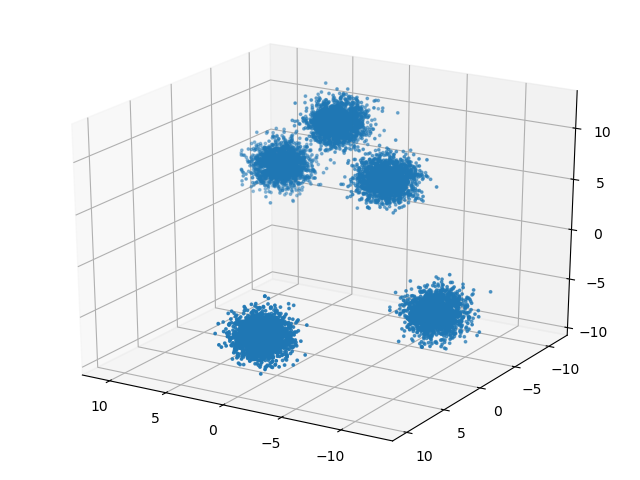
\includegraphics[width=0.92\textwidth]{img/example_not_clustered}
\end{figure}

\vspace{-1cm}

\begin{figure}
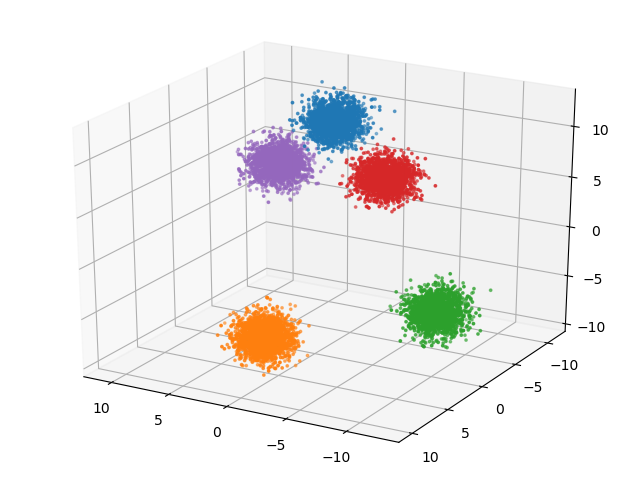
\includegraphics[width=0.92\textwidth]{img/example_clustered}
\end{figure}

\end{columns}
\end{frame}

%----------------------------------------------------------------
%----------------------------------------------------------------

\section{OpenMP}

\begin{frame}
\frametitle{OpenMP implementation}
\begin{columns}[c]

\column{0.5\textwidth}
\begin{algorithm}[H]
\tiny
\caption{OpenMP Mean shift core}
\label{OpenMPAlgorithm}
\begin{algorithmic}
\Function{OpenMPMeanShift}{$originalPoints$}
	\State$shiftedPoints \gets originalPoints$
    \While{iterationIndex $<$ $MAX\_ITERATIONS$}
    			\State \colorbox{lime!30}{\#pragma parallel for schedule(static)}
            \For{each point $p$ in $shiftedPoints$}
               \State $p\gets \Call{ShiftPoint}{p, originalPoints}$
            \EndFor
    \EndWhile
\EndFunction
\end{algorithmic}
\end{algorithm}

\begin{algorithm}[H]
\tiny
\caption{Shift a single point}
\label{ShiftPointAlgSeq}
\begin{algorithmic}
\Function{ShiftPoint}{$p, originalPoints$}
	\State $shiftedP\gets0$
	\State $weight\gets0$
    \For{each point $x$ in $originalPoints$}
    		\State$dist \gets dist(p, x)$
    		\State $w \gets GKernel(dist, BW)$
    		\State $shiftedP \gets shiftedP + w*x$
    		\State $weight \gets weight + w$
    \EndFor
    \State \textbf{return} $shiftedP/weight$
\EndFunction

\end{algorithmic}
\end{algorithm}

\column{0.5\textwidth}
\begin{itemize}
\item just a pragma directive
\vspace{0.75cm}
\item static scheduling: loop divided statically in chunks of equal size
\end{itemize}

\end{columns}
\end{frame}

%----------------------------------------------------------------
%----------------------------------------------------------------

\section{CUDA}

\begin{frame}
\frametitle{Exploiting GPUs: CUDA}
Taking advantage of GPUs:
\vspace{0.45cm}
\begin{itemize}
\item One thread for each point to shift
\vspace{0.35cm}
\item Coalescing of accesses to memory:
\vspace{0.25cm}
\begin{itemize}
\item Points stored as a \emph{Structure of Arrays}
\begin{align}
[x_{}, \ldots , x_{n}, y_{1}, \ldots, y_{n}, z_{1}, \ldots , z_{n}]
\end{align}
\item Access to the array in the form of:
\begin{align}
blockDim.x*blockIdx.x+threadIdx.x
\end{align}
\end{itemize}
\end{itemize}
\end{frame}

%----------------------------------------------------------------
%----------------------------------------------------------------

\subsection{Naive version}

\begin{frame}
\frametitle{Naive CUDA implementation}
\begin{columns}

\column{.4\textwidth}
\tiny{
\begin{algorithm}[H]
\tiny
\caption{CUDA Naive version Mean Shift core}
\label{NaiveCUDAMeanShiftAlg}
\begin{algorithmic}
\Function{NaiveCUDAMS}{$originalPoints$}
	\State$shiftedPoints \gets originalPoints$
    \While{iterationIndex $<$ $MAX\_ITERATIONS$}
    		\State $\Call{NaiveKernel}{shiftedPoints, originalPoints}$
    \EndWhile
\EndFunction
\end{algorithmic}
\end{algorithm}
}

\column{.6\textwidth}

\begin{algorithm}[H]
\tiny
\caption{CUDA Naive version Kernel}
\label{NaiveCUDAKernelAlg}
\begin{algorithmic}
\Function{NaiveKernel}{$shiftedPts, originalPts$}
	\State $tx \gets threadIdx.x$
	\State $bx \gets blockIdx.x$
	\State $idx \gets bx * blockDim.x + tx$
	\If{$idx < |originalPts|$}
	\State $shiftedP \gets 0$
	\State $weight \gets 0$
	\State $p \gets shiftedPts[idx]$
    \For{each point $x$ in $originalPts$}
    		\State$dist \gets dist(p, x)$
    		\State $w \gets GKernel(dist, BW)$
    		\State $shiftedP\gets shiftedP + w*x$
    		\State $weight \gets weight + w$
    \EndFor
    \State $shiftedPts[idx] \gets shiftedP/weight$
    \EndIf
\EndFunction
\end{algorithmic}
\end{algorithm}

\end{columns}

\end{frame}

%----------------------------------------------------------------
%----------------------------------------------------------------

\subsection{Tiling version}

\begin{frame}
\frametitle{Tiling CUDA}
A further optimization is possible:
\vspace{0.45cm}
\begin{itemize}
\item Each thread reads \emph{O(n)} points from global memory to compute the shift
\vspace{0.25cm}
\item Shared Memory can be exploited with the Tiling pattern
\vspace{0.25cm}
\item $TILE\_WIDTH$ = $BLOCK\_DIM$
\vspace{0.25cm}
\item \emph{O(n)} accesses reduced to \emph{O(n/$TILE\_WIDTH$)}
\end{itemize}
\end{frame}

%----------------------------------------------------------------
%----------------------------------------------------------------

\begin{frame}
\frametitle{Tiling CUDA implementation}
\begin{columns}[c]
\column{.4\textwidth}

\tiny{
\begin{algorithm}[H]
\tiny
\caption{\small{CUDA Tiling version Mean Shift core}}
\label{TilingCUDAMeanShiftAlg}
\begin{algorithmic}
\Function{TilingCUDAMS}{$originalPoints$}
	\State$shiftedPoints \gets originalPoints$
    \While{iterationIndex $<$ $MAX\_ITERATIONS$}
    		\State $\Call{TilingKernel}{shiftedPoints, originalPoints}$
    \EndWhile
\EndFunction
\end{algorithmic}
\end{algorithm}
}

\column{.6\textwidth}
\vspace{-0.45cm}
\begin{algorithm}[H]
\tiny
\caption{CUDA Tiling version Kernel}
\label{TilingCUDAKernelAlg}
\begin{algorithmic}
\Function{TilingKernel}{$shiftedPts, originalPts$}
	\State $tx \gets threadIdx.x$
	\State $bx \gets blockIdx.x$
	\State $idx \gets bx * blockDim.x + tx$
	\State $tile \gets SharedMemArray[TILE\_WIDTH]$
	\State $shiftedP \gets 0$
	\State $weight \gets 0$
	\For{$tileIter < numTiles$}
		\State$tileIdx \gets tileIter * TILE\_WIDTH + tx$
		\If{$idx < |originalPts|$}
			\State$tile[tx] \gets originalPts[tileIdx]$
		\Else
			\State$tile[tx] \gets nullPoint$
		\EndIf
		\State $\_\_synchthreads()$\Comment{End of loading}
		\If{$idx < |originalPts|$}
			\State $p \gets shiftedPts[idx]$
    			\For{$i$ with $i < TILE\_WIDTH$}
    				\State $x \gets tile[i]$
    				\If{$x != nullPoint$}
    					\State $dist \gets dist(p, x)$
    					\State $w \gets GKernel(dist, BW)$
    					\State $shiftedP\gets shiftedP + w*x$
    					\State $weight \gets weight + w$
    				\EndIf
    			\EndFor
    		\EndIf
    		\State $\_\_synchthreads()$\Comment{End of computing}
	\EndFor
	\If{$idx < |originalPts|$}
    		\State $shiftedPts[idx] \gets shiftedP/weight$
    	\EndIf
    
\EndFunction
\end{algorithmic}
\end{algorithm}
\end{columns}
\end{frame}

%----------------------------------------------------------------
%----------------------------------------------------------------

\section{Experimental results}

\begin{frame}
\frametitle{Experimental results}
\begin{itemize}
\item Performances compared with the speedup metric, computed as:
\begin{align}
S = \dfrac{t_S}{t_P}
\end{align}
\item Tests executed on a machine with:
\vspace{0.15cm}
\begin{itemize}
\item OS: Ubuntu 18.04 LTS
\vspace{0.05cm}
\item CPU: Intel Core i7-8565U 1.8GHz up to 4.6GHz with Turbo Boost, 4 cores/8 threads
\vspace{0.05cm}
\item RAM: 16 GB DDR4
\vspace{0.05cm}
\item GPU: NVidia GeForce MX250 2GB with CUDA 10.1
\end{itemize}
\vspace{0.25cm}
\item Each time is the average of 5 experiments for the sequential and OpenMP versions and of 15 experiments for both CUDA implementations
\end{itemize}
\end{frame}

%----------------------------------------------------------------
%----------------------------------------------------------------

\begin{frame}
\frametitle{Experimental results (cont.)}
\begin{itemize}
\item The implementations have been evaluated on gaussian distributions composed by respectively 100, 1000, 10000, 100000 and 250000 3D points
\vspace{0.45cm}
\item bandwidth set to 2
\vspace{0.45cm}
\item $MAX\_ITERATIONS$ constant set to 10, which has been empirically estimated to be enough to make all points converge to the local maxima
\end{itemize}

\end{frame}

%----------------------------------------------------------------
%----------------------------------------------------------------

\subsection{OpenMP}

\begin{frame}
\frametitle{OpenMP: Increasing threads}
%\vspace{-0.9cm}
Number of threads gradually increased for each dataset
\vspace{0.25cm}

\begin{columns}[c]

\column{0.5\textwidth}

\vspace{-0.5cm}

\begin{figure}
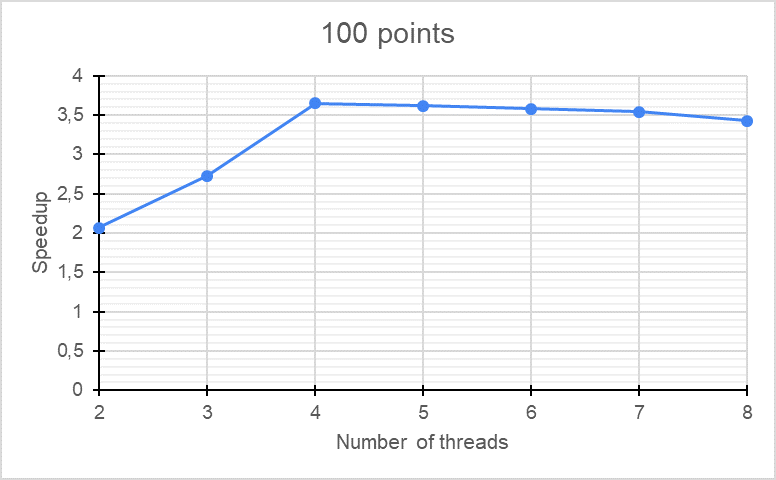
\includegraphics[width=0.7\textwidth]{img/chart_100_points}
\end{figure}

\vspace{-0.5cm}

\begin{figure}
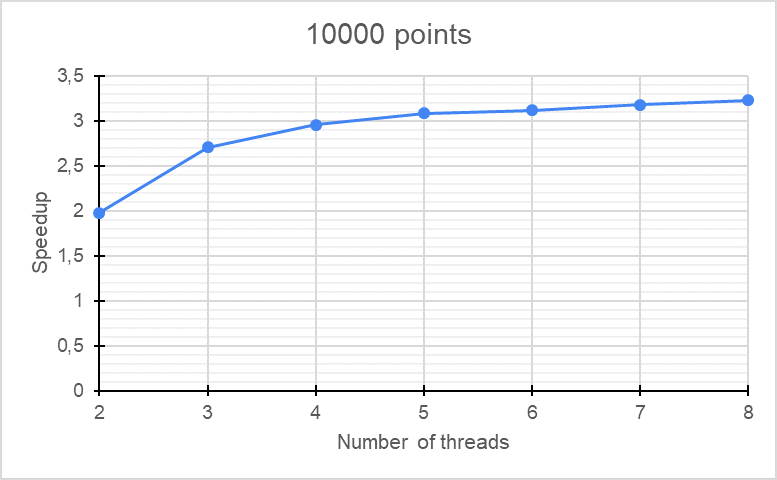
\includegraphics[width=0.7\textwidth]{img/chart_10000_points}
\end{figure}

\column{0.5\textwidth}

\vspace{-0.5cm}

\begin{figure}
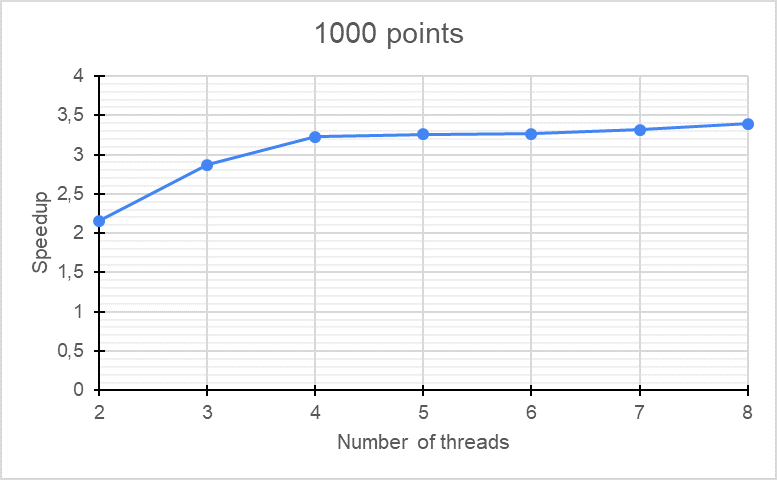
\includegraphics[width=0.7\textwidth]{img/chart_1000_points}
\end{figure}

\vspace{-0.5cm}

\begin{figure}
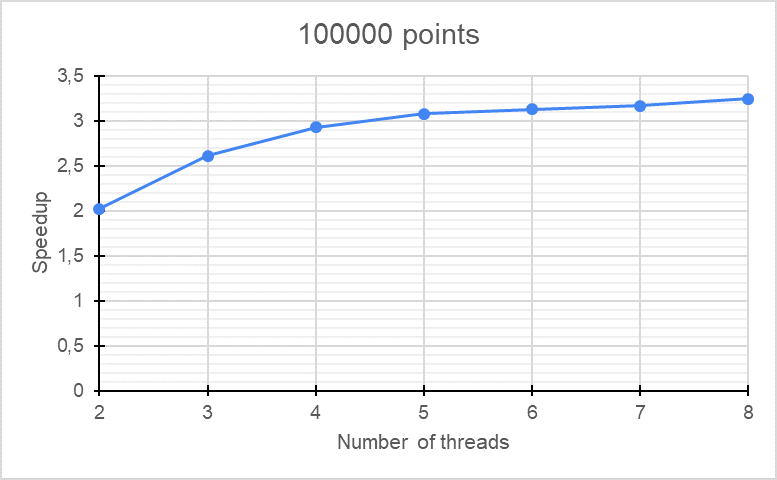
\includegraphics[width=0.7\textwidth]{img/chart_100000_points}
\end{figure}

\end{columns}

\vspace{0.4cm}
Not tested on 250k points dataset: too long execution time

\end{frame}

%----------------------------------------------------------------
%----------------------------------------------------------------

\subsection{CUDA}

\begin{frame}
\frametitle{Tiling CUDA: $TILE\_WIDTH$}
Execution time for 10000 points for the CUDA tiling implementation varying $TILE\_WIDTH$
\begin{columns}[c]
\column{.5\textwidth}

\begin{figure}
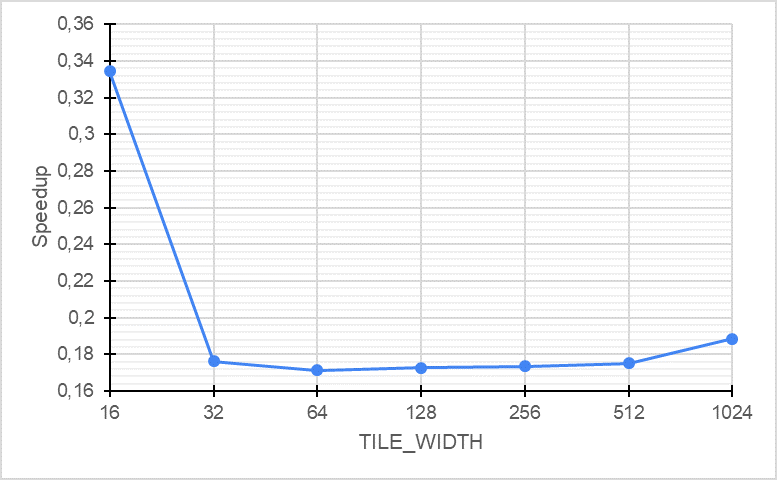
\includegraphics[width=0.99\linewidth]{img/chart_tile_width}
\label{fig:chartTileWidth}
\end{figure}

\column{.5\textwidth}

\begin{table}[]
\centering
\begin{tabular}{|c|c|}
\hline
\textbf{\textbf{TILE$\_$WIDTH}} & \textbf{CUDA Tiling} \\ \hline
16 & 0.334405 s \\ \hline
32 & 0.176171 s \\ \hline
\textbf{64} & \textbf{0.171354 s} \\ \hline
128 & 0.172666 s \\ \hline
256 & 0.173306 s \\ \hline
512 & 0.175091 s \\ \hline
1024 & 0.18845 s \\ \hline
\end{tabular}
\label{tab:tableCudaSpeedup}
\end{table}
\end{columns}
\end{frame}

%----------------------------------------------------------------
%----------------------------------------------------------------

\begin{frame}
\frametitle{Naive vs Tiling CUDA}
\begin{table}[]
\centering
\begin{tabular}{|c|c|c|c|}
\hline
\textbf{Dim} & \textbf{CUDA Naive} & \textbf{CUDA Tiling} & \textbf{Speedup} \\ \hline
100 & 0.000401 s & 0.000437 s & 1.09 \\ \hline
1000 & 0.003044 s & 0.003359 s & 1.11 \\ \hline
10000 & 0.171354 s & 0.191216 s & 1.12 \\ \hline
100000 & 15.79 s & 18.29 s & 1.16 \\ \hline
250000 & 100.38 s & 121.10 s & 1.20 \\ \hline
\end{tabular}
\label{tab:naiveTilingSpeedup}
\end{table}
\end{frame}

%----------------------------------------------------------------
%----------------------------------------------------------------

\begin{frame}
\frametitle{Tiling CUDA speedup}
\begin{table}[]
\centering
\begin{tabular}{|c|c|c|c|}
\hline
\textbf{Dim} & \textbf{Sequential} & \textbf{CUDA Tiling} & \textbf{Speedup} \\ \hline
100 & 0.005384 s & 0.000401 s & 13.43 \\ \hline
1000 & 0.475485 s & 0.003044 s & 156.21 \\ \hline
10000 & 49.29 s & 0.171354 s & 287.64 \\ \hline
100000 & 4560.37 s & 15.79 s & 288.80 \\ \hline
250000 & $\dagger$ 27768 s & 100.38 s & $\dagger$ 276.61 \\ \hline
\end{tabular}
\label{tab:cudaSpeedup}
\end{table}
\vspace{0.35cm}

\begin{itemize}
\item $\dagger$ time has been estimated with a quadratic regression (due to the $O(n^{2})$ computational cost)
\end{itemize}

\end{frame}



%----------------------------------------------------------------
%----------------------------------------------------------------

\subsection{Global comparison}

\begin{frame}
\frametitle{Global comparison}

Global comparison between sequential, OpenMP and Tiling CUDA best results:
\vspace{0.25cm}
\begin{itemize}
\item Greatest speedups with CUDA, at the expense of a more complicated implementation
\vspace{0.15cm}
\item OpenMP lets to reach noticeable speedups with a simple implementation (just a directive)
\end{itemize}
\vspace{0.25cm}

\centering
\begin{table}[]
\resizebox{0.99\linewidth}{!}{
\begin{tabular}{|c|c|c|c|c|c|c|}
\hline
\textbf{Dim} & \multicolumn{2}{c|}{\textbf{Sequential}} & \textbf{OpenMP} & \textbf{OpenMP Speedup} & \textbf{CUDA Tiling} & \textbf{CUDA Speedup} \\ \hline
100 & \multicolumn{2}{c|}{0.005384 s} & 0.001473 s & 3.66 & 0.000401 s & 13.43 \\ \hline
1000 & \multicolumn{2}{c|}{0.475485 s} & 0.140161 s & 3.39 & 0.003044 s & 156.21 \\ \hline
10000 & \multicolumn{2}{c|}{49.29 s} & 15.25 s & 3.24 & 0.171354 s & 287.64 \\ \hline
100000 & \multicolumn{2}{c|}{4560.37 s} & 1403.78 s & 3.25 & 15.79 s & 288.80 \\ \hline
250000 & \multicolumn{2}{c|}{$\dagger$ 27768 s} & $\dagger$ 8720 s & $\dagger$ 3.18 & 100.38 s & $\dagger$ 276.61 \\ \hline
\end{tabular}}
\caption{$\dagger$ times have been estimated with a quadratic regression}
\label{tab:globalComparison}
\end{table}
\end{frame}

%----------------------------------------------------------------
%----------------------------------------------------------------

\section{Conclusions}

\begin{frame}
\frametitle{Conclusions}
\begin{itemize}
\item The embarassingly parallel structure of Mean Shift makes it suitable for parallel implementations
\vspace{0.45cm}
\item OpenMP has an excellent speedup and development cost ratio
\vspace{0.45cm}
\item CUDA makes Mean Shift applicable to datasets intractable with a CPU
\end{itemize}
\end{frame}

\end{document} 